%%%%%%%%%%%%%%%%%%%%%%% file typeinst.tex %%%%%%%%%%%%%%%%%%%%%%%%%
%
% This is the LaTeX source for the instructions to authors using
% the LaTeX document class 'llncs.cls' for contributions to
% the Lecture Notes in Computer Sciences series.
% http://www.springer.com/lncs       Springer Heidelberg 2006/05/04
%
% It may be used as a template for your own input - copy it
% to a new file with a new name and use it as the basis
% for your article.
%
% NB: the document class 'llncs' has its own and detailed documentation, see
% ftp://ftp.springer.de/data/pubftp/pub/tex/latex/llncs/latex2e/llncsdoc.pdf
%
%%%%%%%%%%%%%%%%%%%%%%%%%%%%%%%%%%%%%%%%%%%%%%%%%%%%%%%%%%%%%%%%%%%
\documentclass[runningheads,a4paper]{llncs}

\usepackage[colorlinks=true,citecolor=blue]{hyperref}
\usepackage{amsmath,amssymb}
\setcounter{tocdepth}{3}

\usepackage{graphicx}
\graphicspath{ {images/} }

\usepackage{multirow}
\usepackage{url}
\usepackage{verbatim}

\urldef{\mailsa}\path|rcha9612@uni.sydney.edu.au, aditya.menon@data61.csiro.au, schawla@qf.org.qa|

\newcommand{\keywords}[1]{\par\addvspace\baselineskip
\noindent\keywordname\enspace\ignorespaces#1}

\usepackage{subfigure}
\usepackage{multirow}
\usepackage{soul,color,colortbl}
\usepackage{xcolor}
\usepackage{booktabs}
\usepackage{upgreek}

\newcommand{\A}{\mathbf{A}}
\newcommand{\B}{\mathbf{B}}
\newcommand{\E}{\mathbf{E}}
\newcommand{\I}{\mathbf{I}}
\newcommand{\J}{\mathbf{J}}
\newcommand{\N}{\mathbf{N}}
\newcommand{\R}{\mathbf{R}}
\renewcommand{\S}{\mathbf{S}}
\newcommand{\T}{\mathbf{T}}
\newcommand{\U}{\mathbf{U}}
\newcommand{\V}{\mathbf{V}}
\newcommand{\W}{\mathbf{W}}
\newcommand{\X}{\mathbf{X}}
\newcommand{\Z}{\mathbf{Z}}

\newcommand{\Real}{\mathbb{R}}
\newcommand{\sanjay}[1]{\hl{\footnote{\hl{Sanjay: #1}}}}

\let\oldFootnote\footnote
\newcommand\nextToken\relax

\renewcommand\footnote[1]{%
    \oldFootnote{#1}\futurelet\nextToken\isFootnote}

\newcommand\isFootnote{%
    \ifx\footnote\nextToken\textsuperscript{,}\fi}

\begin{document}

\mainmatter  % start of an individual contribution

% first the title is needed
\title{Robust, Deep and Inductive Anomaly Detection}

% a short form should be given in case it is too long for the running head
\titlerunning{Robust, Deep and Inductive Anomaly Detection}

% the name(s) of the author(s) follow(s) next
%
% NB: Chinese authors should write their first names(s) in front of
% their surnames. This ensures that the names appear correctly in
% the running heads and the author index.
%
\author{Raghavendra Chalapathy\inst{1} \and Aditya Krishna Menon\inst{2} \and Sanjay Chawla\inst{3}}

%
\authorrunning{Chalapathy, Menon and Chawla}
% (feature abused for this document to repeat the title also on left hand pages)

% the affiliations are given next; don't give your e-mail address
% unless you accept that it will be published
\institute{University of Sydney and Capital Markets Cooperative Research Centre (CMCRC)
\and 
Data61/CSIRO and the Australian National University
\and
Qatar Computing Research Institute \\
\mailsa\\
 }

%
% NB: a more complex sample for affiliations and the mapping to the
% corresponding authors can be found in the file "llncs.dem"
% (search for the string "\mainmatter" where a contribution starts).
% "llncs.dem" accompanies the document class "llncs.cls".
%

\toctitle{Lecture Notes in Computer Science}
\tocauthor{Authors' Instructions}
\maketitle


\begin{abstract}
%!TEX root = ../main.tex
Anomaly detection is an important problem that has been well-studied within diverse research areas and application domains. The aim of this survey is two fold, firstly we present a structured and comprehensive overview of research methods in deep learning-based anomaly detection. Furthermore, we review the adoption of these methods for anomaly across various application domains and asess their effectiveness. We have grouped state-of-the-art research techniques into different categories based on the underlying assumptions and approach adopted.  Within each category we outline the basic anomaly detection technique, alongwith its variants and present key assumptions, to differentiate between normal and anomalous behavior. For each category we present we also present the advantages and limitations and discuss the computational complexity of the techniques in real application domains. Finally, we outline open issues in research and challenges faced while adopting these techniques.


\end{abstract}

\section{Anomaly detection: motivation and challenges}
%%%%%%%%%%%%%%%%%%%%%%%%%%%%%%%%%%%%%%%%%%%%%%%%%%%%%%%%%%%%%%%%%%%%%%%%%
%
%	LaTeX File for Stanford University PhD Thesis
%
%%%%%%%%%%%%%%%%%%%%%%%%%%%%%%%%%%%%%%%%%%%%%%%%%%%%%%%%%%%%%%%%%%%%%%%%%
%	Copyright 2001  by  Jung-Suk Goo    (goojs@gloworm.stanford.edu)
%%%%%%%%%%%%%%%%%%%%%%%%%%%%%%%%%%%%%%%%%%%%%%%%%%%%%%%%%%%%%%%%%%%%%%%%%

\chapter{Introduction}

%%%%%%%%%%%%%%%%%%%%%%%%%%%%%%%%%%%%%%%%%%%%%%%%%%%%%%%%%%%%%%%%%%%%%%%%
%\section{Introduction} 
% allow  = 	permit, let, authorize, grant, empower, enable, entitle, qualify, agrees, offer, provide, express, show, assign, allocate, produce, construct, create, generate, induce, instigate, promote

% consistent = steady, stable, constant, regular, even, uniform, orderly, unchanging, unvarying, unswerving, undeviating, unwavering, unfluctuating, homogeneous, true to type; dependable, reliable, unfailing, predictable, reliable

% detect = 	identify, distinguish, establish, deduce, determine, differentiate, discriminate, discern, separate, characterise, discover, uncover, find, find out, turn up,  expose, reveal

% use = utilize, make use of, avail oneself of, employ, work, operate, wield, ply, apply, manoeuvre, manipulate,

%% In the introduction - do not explain any methods that are central to the comparison study
% Why Should we care?
%Background on group analysis - define group and explain, why are group interesting?
%
%1. Background.
%In this part you have to make clear what the context is. Ideally, you should give an idea of the state-of-the art of the field the report is about. But keep it short: in my opinion this part should be less than a page long. 
%Application motivation

%At the close of 2012, the monetary value of the world stock market was about US\$55 trillion.
Pointwise anomaly and change detection focus on the study of individual data instances that do not conform with the expected pattern in a dataset. With the increasing availability of multifaceted information, there is a growing trend in research involving groups or collections of observations. For example,  
 Muandet et al.	\cite{OCSMM} possibly detect Higgs bosons as a group of collision events  in high energy particle physics while a group of multiple sensor networks in Chen and Yu \cite{chen2016collaborative}, allow for a robust  detection of  distributed denial-of-service attacks. Group deviation detection  techniques achieve fewer false positives than pointwise approaches as a greater number of observations occur in group applications. %provide a better characterization of group behaviors. 
  Many pointwise anomaly detection methods are also not compatible  in detecting  group deviations so we turn to more specialized techniques.  
 



 

Group deviation detection involves the discovery of group behaviors which significantly deviate from the expected group patterns.   In particular, group anomaly detection (GAD) is the process of identifying groups that are not consistent with regular group patterns while group change detection (GCD) estimates significant deviations in the state of a group over  time. GAD and GCD methods achieve a higher performance  than pointwise methods for detecting group deviations. Even though GAD usually involves time-independent  applications and GCD relates to time-dependent groups, both problems share a common framework  and similar fundamental ideas.  
This survey  elaborates on group deviation detection techniques in static and dynamic situations. 

%Groups are also synonymous with collections, clusters or communities. 
%The terms group anomalies  and group outliers are interchangeable however we use group anomalies or anomalous groups in this survey.
 
% are synonymous with group outliers but  are also a specific type of collective contextual anomalies.    %Groups are defined according to different  contexts  where a group is a cluster of galexies in an astronomical dataset %\cite{OCSMM} ,MGM,FGM,GLAD}.
  %Group anomaly detection is the process of discovering patterns in groups that are not consistent with the expected behavior \cite{Chandola}. 

% emerging area of research


%Imagine a series of events leads to a financial butterfly effect and many portfolios of  stocks in the market require immediate asset reallocation. 


%groups exhibiting irregular behavior may represent a disease outbreaks  to malicious web spammers.  

  

%	  politics \cite{GLAD} 
  %Images in a photo album & Distortion \\

 
 
%Many papers mainly analyze the static natures of groups, however it is also interesting to monitor the evolution of groups over time. This is where multivariate time series and changepoint detection are applied.

% Group Distribution
%In our study, we focus on group behaviors based on numerical data. 




% \subsection{Definition of Groups} %
A group is a collection of two or more related data instances.    %F\~{a}rber et al. \cite{ClusterEval} even discusses how known group labels may not correspond to inherently clustered points. 
In GAD, a group anomaly has  significantly different  statistical properties  with respect to multiple groups whereas GCD involves detecting  a significant change   in a group  with respect to past group observations.   Group structures may be known a priori such as words in a documents otherwise when group   memberships between instances in a dataset are unknown, additional information or clustering algorithms are required. 
  Thus the initial definition of groups affects subsequent analysis and results. 
  %The validity of interpretations of known group labels and inherent clusters is discussed in  .   



 
    
   
More specifically,  Xiong et al.  \cite{MGM} categorize group deviations as either point-based or distribution-based for GAD applications.   Point-based anomalous groups are where all of the members are also pointwise anomalies. Similarly in GCD, a point-based group change signifies that time series in a group over time also experience significant changes.   On the other hand, a  distribution-based group anomaly  is where a collection of points differs from expected group patterns, however individual data instances may not seem anomalous. Likewise, a distribution-based change in a group over time occurs when individual time series exhibit regular behavior however their collective pattern is significantly different.   

 % between multiple variables. 
  
%  %  groups are represented by a set of features. %descriptive properties. 
%One way of specifying features of a group is through statistical properties of group distributions  such as location, scale, shape and dependence between multiple variables.   %Other  descriptive properties of a group % distributions 
%Other descriptions of group features such as rules and network connections are dependent on the availability of data. 
 
 

  %Their study investigates examples of Gaussian mixtures where a group anomaly is generated from a different proportion of distributions. 

%In these cases,  individual data instances exhibit regular behavior however the collective behaviors of roup 3 are anomalous in Figure \ref{Fig:Intro}. Since there are a variety of statistical properties for a group distribution, it is difficult to robustly capture anomalous behaviors using pointwise anomaly detection methods.





 %We focus on measures of distributions in terms of location, scale, shape and dependence between multiple variables. Different detection techniques have a better performance for particular anomalous patterns. 
  %  Thus our research analyzes a variety of  statistical properties as described in Table \ref{Tab:Des}. Most group anomaly detection methods are interested in distribution-based anomalies which are 




%\begin{figure}[H]
%\centering
% \begin{subfigure}[b]{0.6\textwidth}
%                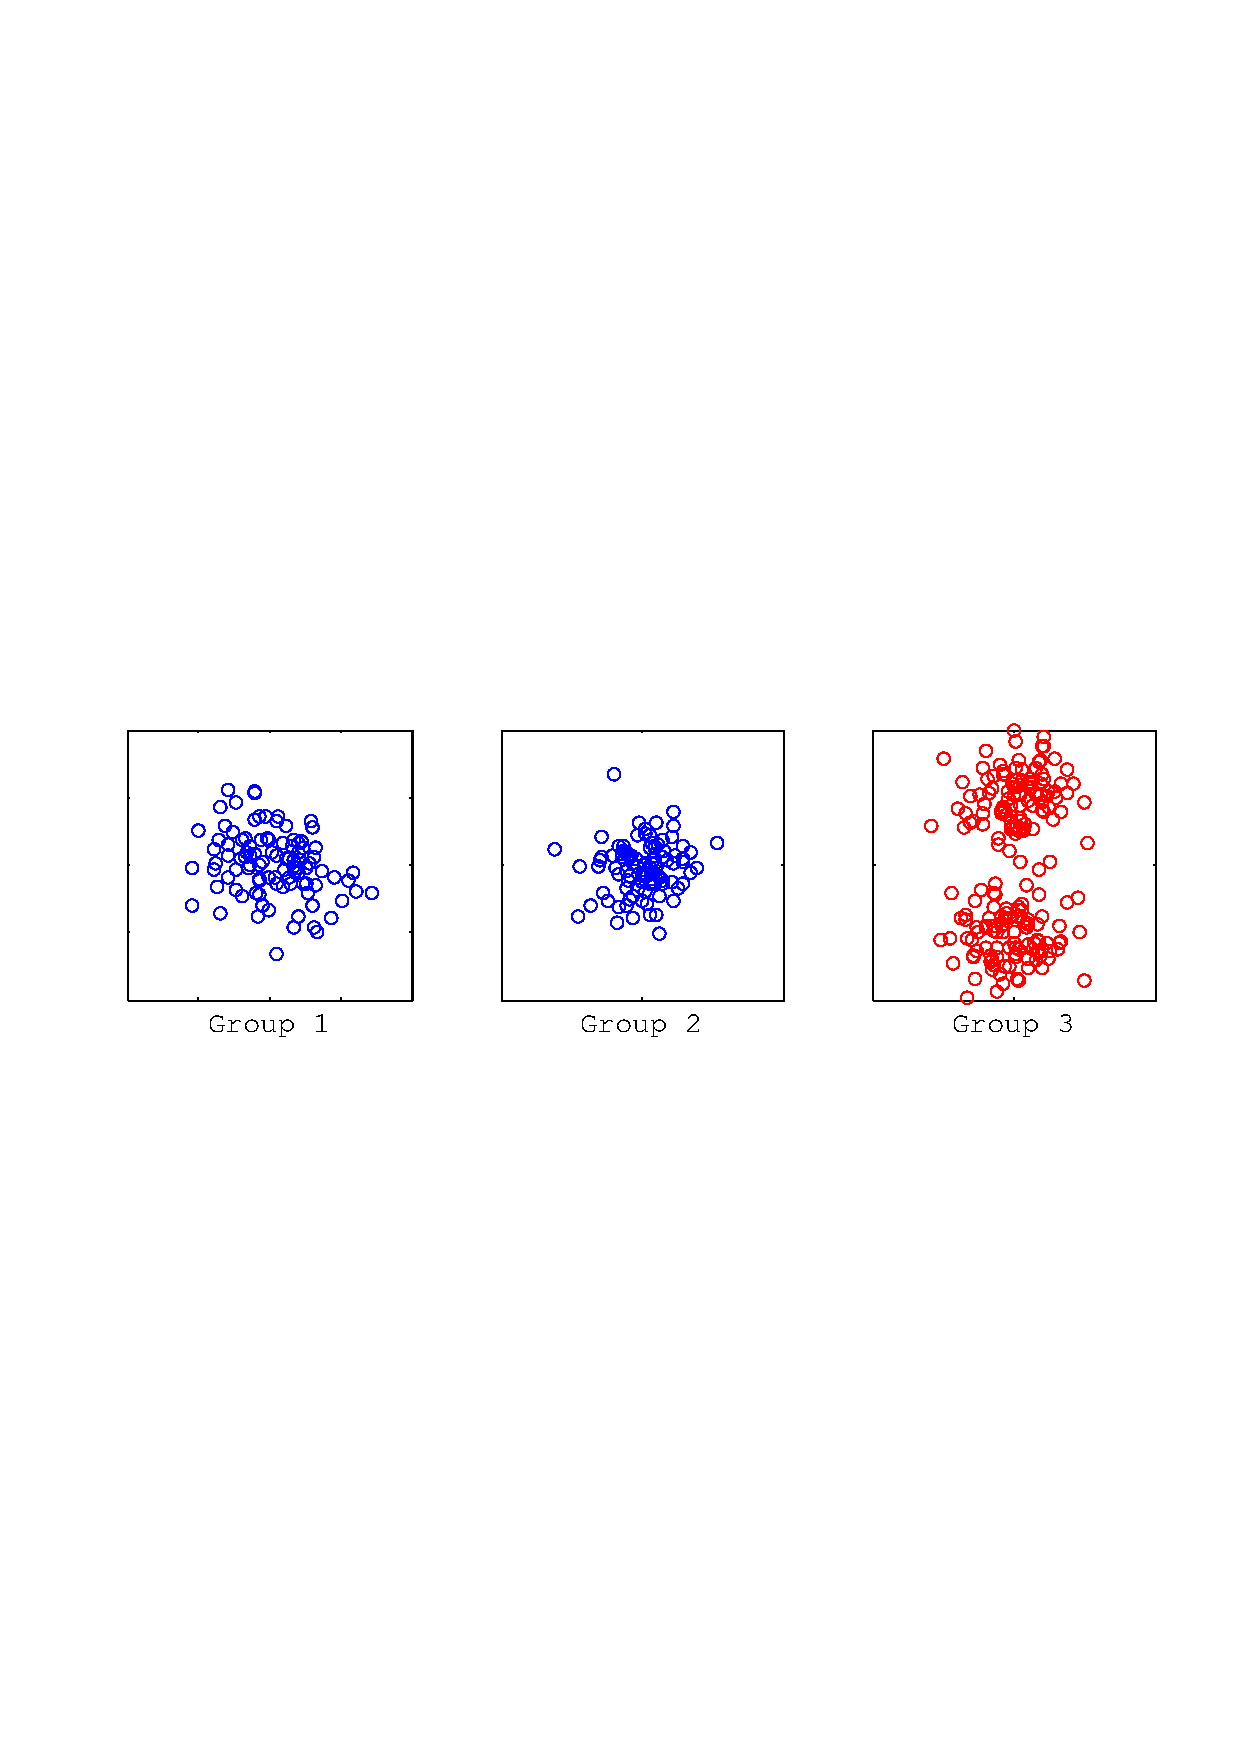
\includegraphics[width=\linewidth,trim=3cm 12cm 3cm 11.5cm]{Ex1}
%                \caption{A significant deviation in scale or shape.}
%        \end{subfigure}%
%        \hfill
% \begin{subfigure}[b]{0.6\textwidth}
%                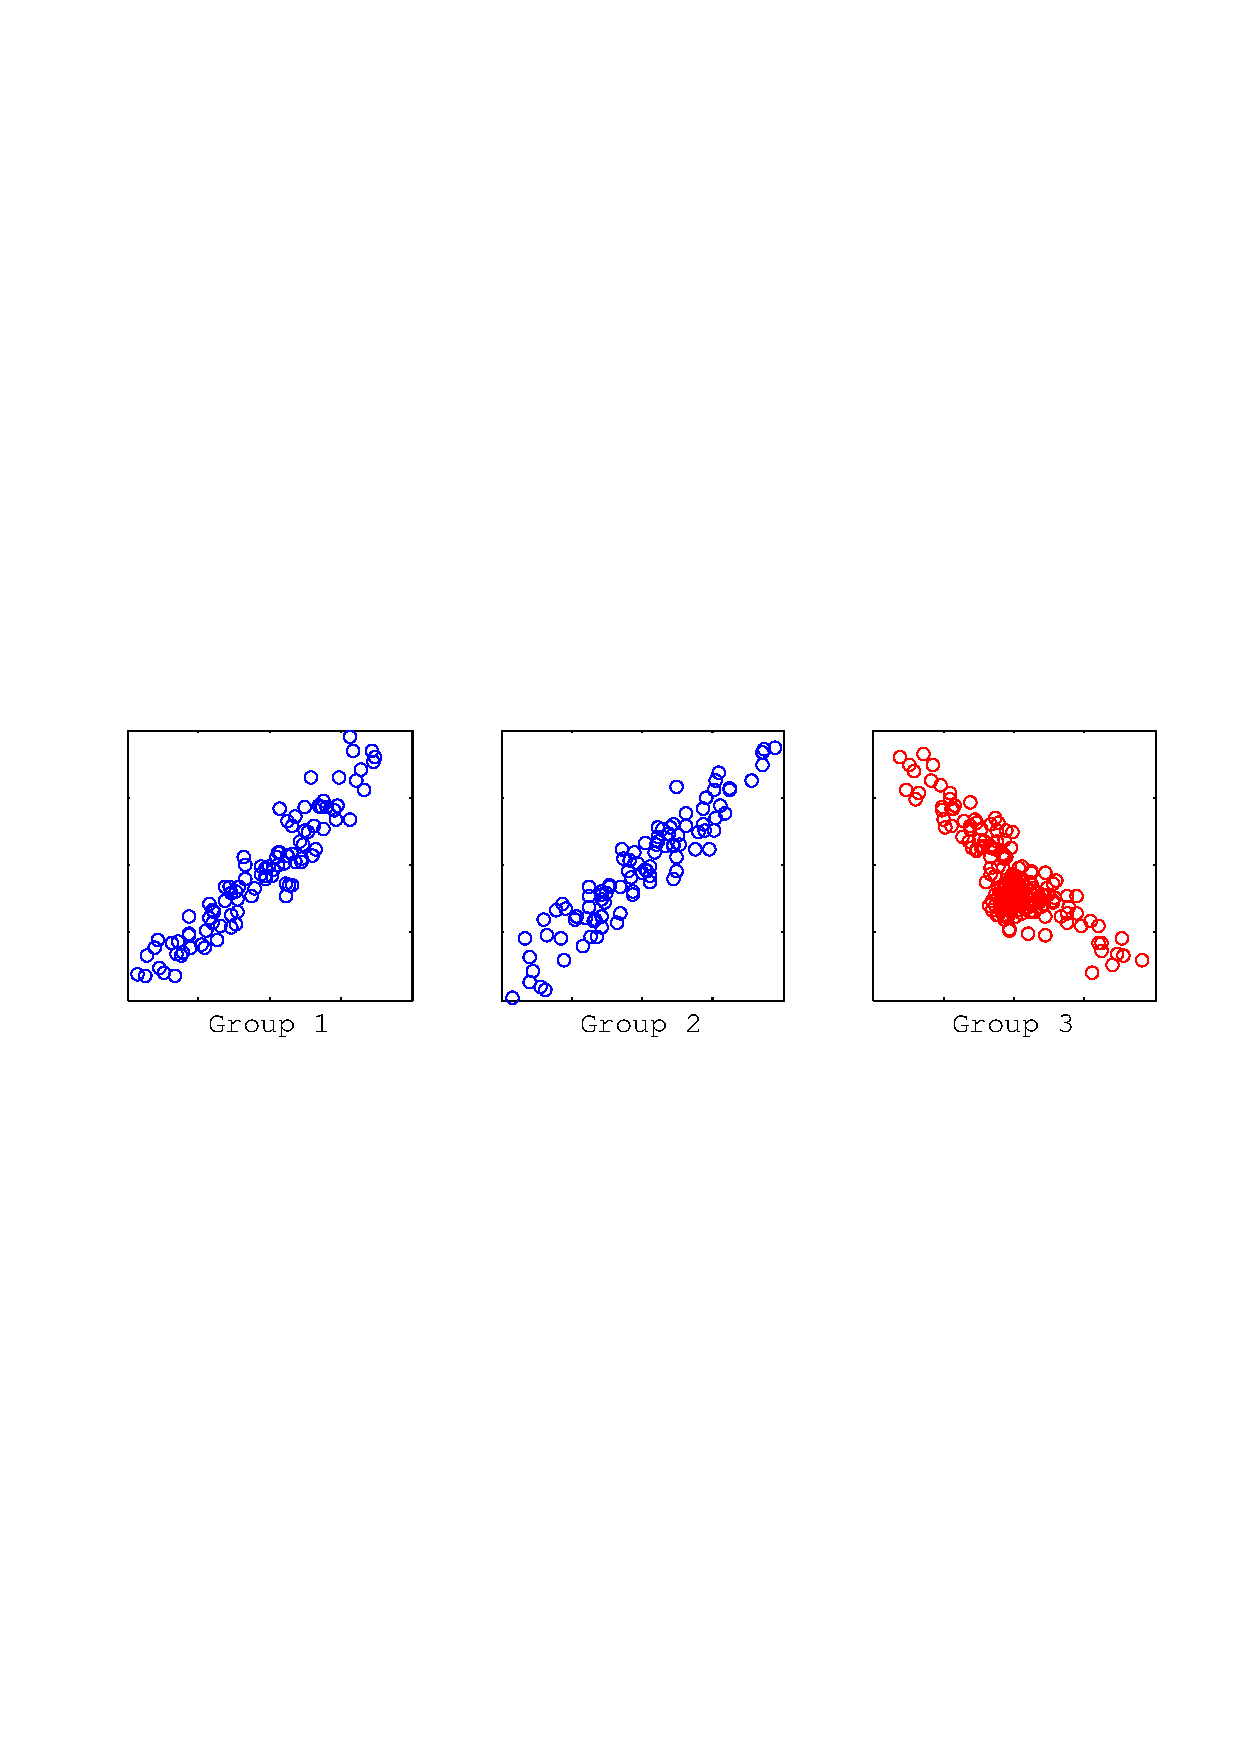
\includegraphics[width=\linewidth,trim=3cm 12cm 3cm 11.5cm]{Ex2}
%                \caption{Significant deviation in covariance or correlation. }
%  \end{subfigure}%
%%\includegraphics[width=7.5cm, height=5.2cm,trim=3cm 9cm 3cm 10cm]{ToyExample}
%\caption{Examples of group behaviors that clearly deviate in terms of different statistical properties; (a) scale or shape and (b) covariance or correlation.  
%}
%\label{Fig:Intro}
%\end{figure} 


 Figure \ref{Fig:Intro} highlights two examples where distribution-based group deviations are characterized by two different statistical properties. The first row in (a) illustrates Group 3 with a relatively greater  scale or shape whereas in the second row (b),  a Group 3 is characterized by a rotated covariance or correlation structure between variables. 
 % Depending on the context, Group 3 in each row of Figure \ref{Fig:Intro} may represent   a group anomaly for a GAD application whereas in a GCD context, Group 3 is a time-dependent group where a significant change in group occurs at $t=3$.  
  {  
  Depending on the specific domain, the group deviation (Group 3) in  Figure \ref{Fig:Intro} has different interpretations. In Xiong et al. \cite{MGM}, a group anomaly represents an anomalous galaxy with a significantly different scale or shape parameter whereas Chen et al. \cite{GLETS}  examine a GCD context where a significant deviation in correlation between stocks occurs over time.     
    }

%\subsection{Applications}
%By considering a group rather than an individual instance is  beneficial in a diverse range of applications.
 GAD and GCD  techniques provide meaningful insights that are not effectively detected by pointwise  methods  in a diverse range of applications.  
In intrusion detection,  Chen and Yu \cite{chen2016collaborative} explore  a collaborative detection system involving multiple sensor networks to detect distributed denial-of-service attacks. Using collective information from multiple intrusion detection system rather than a single system offers a more reliable detection of coordinated attacks. Another example is where Dai et al. \cite{ERACD} analyze an IMDb movie database where anomalous collection of entities contain highly ranked actors that are otherwise not discovered by pointwise detection methods.   Real-world GAD events have also been studied in group psychology such as  high  performance of employee work teams by   Kozlowski and Bell  \cite{kozlowski2003}.  
   %Zhou et al. \cite{Zhou2010}  A Survey of Coordinated Attacks and Collaborative Intrusion Detection}

Investigating group deviations has a variety of interesting domains, especially physical GAD applications.  %that motivate different avenues of research.
In particular,  Muandet et al.	\cite{OCSMM} investigate GAD for physical phenomena in high energy particle physics such as Higgs bosons that are observed as slight excesses in a collection of collision events rather than individual  events. In Guevara et al. \cite{SMDD}, an anomalous galaxy cluster is identified by an irregular proportion of color pixels. Xiong et al. \cite{FGM} also analyze a physical application with 3-dimensional velocity of a fluid from the  JHU turbulence database  
where a group anomaly represents unusual vorticity in  fluid dynamics.  
 

Textual data is also examined in GAD where a document is considered a group of words. 
Yu et al. \cite{GLAD} investigate scientific publications in order to understand the structure of certain research communities. Irregular communities of co-authors possibly reveal unusual research trends.  By analyzing documents from a training set of news articles, Soleimani and Miller \cite{ATD} infer regular topics   such as $`\mathtt{rec.sport.baseball}'$  and $`\mathtt{ talk.politics.misc}'$. An anomalous cluster in this case consists of novel topics that are unobserved in the training corpus such as $`\mathtt{rec.sport.hockey}'$ and $`\mathtt{talk.politics.mideast}'$. Using  textual information from product reviews on Amazon, Mukherjee et al.  \cite{GroupReviewSpam} identify  groups of spammers that collaborative in writing fake reviews. 

%There are many other applications where GAD and GCD techniques offer interesting results. 
  
  A group over time for GCD is also studied across a variety of domains.  Wong et al. \cite{wong-rule} investigate different demographic groups admitted to  emergency departments in hospitals in a major US city.   A significant change in a particular demographic group over time represents an early indication of a potential epidemic and disease outbreak. 
  Chen et al. \cite{GLETS} monitor a group of  time series  in the stock market where after a specific period, the group disbands with dissimilar individual behaviors.     In this case, a group of seemingly uncorrelated time series may also form a more cohesive collection with a higher correlation over time.  Using multiple sensor data, Xie and Siegmund  \cite{xie2013} explore a general problem of sequential change detection in a proportion of time series in a group over time.   In a political application, Yu et al. \cite{GLAD} discover  a large deviation in voting behaviors of a group of US senators around the time of a Democratic party  election.  
  A real-world GCD event has been discovered in five of the largest private health insurers in Chile where they colluded to unfairly reduced  the coverage of healthcare plans over a period of time \cite{Chile}.  

%Thus once a group anomaly is discovered,  an actionable intervention depending on the particular domain may lead to  mitigating health  risks to reduction of unfair monetary losses. 
 Thus there are interesting and meaningful insights that are gained from GAD and GCD applications such as: 
\begin{enumerate}
\item  New research discoveries; 
Higgs bosons in physics \cite{OCSMM}, 
 anomalous galaxy clusters in astronomy  \cite{SMDD},  unusual vorticity in fluid dynamics \cite{FGM}. 
\item  Mitigation of risks: reduce financial losses  \cite{GLETS}, prevent disease outbreaks  \cite{wong-rule}.
\item   Identification of  fraudulent collaborative  activities:  collusion detection \cite{Chile}, fake product reviews on Amazon  \cite{GroupReviewSpam}, % identifies collaborative group of spammers that write .
 intrusion detection for  distributed denial-of-service attacks  \cite{chen2016collaborative}.   
\item  Interesting  explanatory results;   research trends in academic communities   \cite{GLAD},  changes in political voting preferences \cite{GLAD},  
highly ranked actors in IMDb movies   \cite{ERACD}, performance of employee work teams  \cite{kozlowski2003}.  
\end{enumerate}  

   % Table \ref{Tab:Examples} summarizes group applications explored in the literature and provide a basic interpretations of their results.   
   
% 		\begin{table}[H]
%	\tabcolsep=0.2cm  	\renewcommand{\arraystretch}{1.8}
%	\begin{center}
%	\scalebox{0.8}{
%	\begin{tabular}{|p{3.5cm}|c|l|l|l|l }
%	\hline\\[-5mm]
%%Techniques &	
%Authors & \small Application & Group Dataset & Interpretation of  Results %Group Anomalies
%  \\ \hline \\[-5mm] 
%	% Molecular biology  & Irregular protein-protein interaction \cite{MMSB} \\
%%Discriminative Model  & 	
% \small Chen and Yu \cite{chen2016collaborative}&   & Collaborative  Intrusion Detection % System
%    &
%  Distributed denial-of-service   \\
% Muandet et al.	\cite{OCSMM} &   & High Energy Particle Physics  & Signals  containing  Higgs bosons  \\
% Guevara et al.	\cite{SMDD} &  & Sloan Digital Sky Survey  & Irregular cluster of galaxies  \\
%%\hline\\[-6mm] 
%%\small Xiong et al. \cite{MGM}  &	 Sloan Digital Sky Survey & Irregular cluster of galaxies  \\
%% 	\small Xiong et al. \cite{FGM} & Generative Model &
%% Generative Model  &
%\small Xiong et al. \cite{FGM} & GAD & JHU Turbulence Database Cluster  & Unusual vorticity \\%Image of Fluid Motion   & Unusual turbulence   \\ % Image Data  & Stitched images from different scenes  \\
%	\small Yu et al. \cite{GLAD} &  & Scientific Publications & Research trends in communities  \\
%Mukherjee et al.  \cite{GroupReviewSpam} &  &  Amazon reviews  & Groups of manipulative spammers \\ 
% \small Soleimani and Miller \cite{ATD}  &  & 20-Newsgroup Dataset  & Anomalous document collection   
% \\
% 	\small Dai et al. \cite{ERACD} &  &
%	IMDb Movie Database & Highly ranked actors  
%  \\   
%%Kozlowski et al. \cite{kozlowski2003}  
%\hline 
%	\small Yu et al. \cite{GLAD} &  & Political Voting & Changing voting preferences \\
%  \small Wong et al. \cite{wong-rule} 
%& \multirow{2}{*}{GCD} & Emergency Department %Database 
%	 &  Disease outbreaks \\
%     \small Chen et al. \cite{}  &   &  Stock Market Data     & Increased market variability   \\
%  Xie and Siegmund  \cite{xie2013} &   & Sequential Sensor Data & Change detection  in multiple sensors    \\ 
%     [2mm]
%   %Detecting Extreme Rank Anomalous Collections 
%% %Web Host Graph & Web Spammer entities \\
%% 
% \hline
%	 \end{tabular}
%	 }
%	 \smallskip
%	\end{center}
%	 with interpretations of group devi\caption{ Previous studies involving GAD and GCD applicationsations. }
%\label{Tab:Examples}
%\end{table}   


{ 
%\subsection{Our Contributions}
The objective of this survey paper is to provide a clearer understanding and detailed  overview of group deviation detection research.  %anomaly and change detection techniques involving group observations.  
 We first explain GAD techniques  in multiple static groups and then explore dynamic groups for GCD applications. %We also provide an evaluation of each procedure and suggest future research directions where techniques can be further improved. % Since some methods are  specifically design for a particular domain, we elaborate on the different applications for group anomaly detection.
Our  main contributions are  summarized as: %\vspace{-1mm}
\begin{enumerate}
\item {\bf Clearer Understanding:} 
This survey provides an underlying structure for   both group anomaly detection (GAD) and group change detection (GCD) problems.      % Figure \ref{Fig:Framework}  builds upon the anomaly detection from Chandola \cite{Chandola}
\item {\bf Detailed Overview:} 
 We further elucidate the details of state-of-the-art techniques in terms of four key components as described in Section \ref{Sec:Problem}. 
\item {\bf Discussion:} We also discuss the advantages and disadvantages of current GAD and GCD techniques in terms of discriminative methods, generative models  as well as hypothesis tests. 
\end{enumerate}
 
%\section{Organisation}
The rest of the paper is organized as follows. Section \ref{Sec:Framework} describes the underlying structure and ideas relating to group deviation detection.  Section \ref{Sec:Problem}  formalizes the group deviation detection problem where techniques are explained in terms of four key components. Techniques for detecting group anomalies are explained in Section  \ref{Sec:D} while Section \ref{Sec:GCD}  describes methods for detecting significant changes in a group over time. A discussion of our findings and future research for group deviation detection is provided in Section 
 \ref{Sec:Discussion} while Section \ref{Sec:Conclusion} summarizes our survey paper.
}
 

\section{Background and related work on anomaly detection}
\label{sec:background}
\label{sec:related}
% !TEX root=../main.tex
\section{Related Work} \label{DGM:RelatedWork}
GAD is an emerging area  of research where most state-of-the-art techniques have been more recently developed.  While group anomalies are briefly discussed in anomaly detection surveys such as Chandola et al. \cite{Chandola} and Austin \cite{Hodge},  
  Yu et al. \cite{SurveySocialMedia} elaborates on GAD techniques where group memberships are not previously known.  
   {  Recently Toth and Chawla \cite{MySurvey} provide a comprehensive overview of GAD methods as well as a detailed  description of detecting temporal changes in groups over time. 
}
We focus on group anomalies in image applications where group memberships are known a priori. 

Previous studies on image anomaly detection % involving image   applications 
can be understood in terms of group anomalies. 
%Anomaly detection has been  previously studied in a variety of image classification applications. 
Quellec et al.  \cite{mammo} examine mammographic images  where point-based group anomalies represent potentially cancerous regions. Perera and Patel \cite{chairs} learn features from a collection of images containing regular chair objects and detect point-based group anomalies where chairs have abnormal shapes, colors and other irregular characteristics. On the other hand, Xiong et al. \cite{FGM} detect distribution-based group anomalies that are stitched images from scene categories (inside city, mountain or coast). %At a pixel level,   Xiong et al. \cite{MGM} apply GAD methods to detect anomalous galaxy clusters with irregular proportions of RGB pixels. 
We emphasise detecting distribution-based group anomalies rather than point-based anomalies in our subsequent  image applications.

The discovery of group anomalies is of interest to a number of diverse domains.   
  Muandet et al.	\cite{OCSMM} investigate GAD for physical phenomena in high energy particle physics where Higgs bosons are observed as slight excesses in a collection of collision events rather than individual  events. Xiong et al. \cite{FGM} analyse fluid dynamics  where a group anomaly represents unusual vorticity and turbulence in  fluid motion.  % In topic modeling,  Soleimani and Miller \cite{ATD} characterise documents by topics and anomalous clusters of documents are discovered by their irregular  topic mixtures. 
   By incorporating additional information from pairwise connection data, Yu et al. \cite{GLAD} find potentially irregular communities of co-authors in various research communities.
Thus there are many GAD application other than image anomaly detection.
 

A  related discipline to image anomaly detection is video anomaly detection where many DGMs are applied.  
 Sultani  et al.  \cite{survideos1} detect real-world anomalies such as burglary, fighting, vandalism and so on from  CCTV footage using deep learning methods.  %Many techniques involving deep learning architectures have been applied to detect temporal changes in a video surveillance application.    
% In a review, Kiran et al. \cite{survideos2} compare DGMs with different  convolution architectures for  video anomaly detection applications. 
Recent work ~\cite{schlegl2017unsupervised,xu2018unsupervised,an2015variational} illustrate the effectiveness of generative models for high-dimensional anomaly detection. Although, there are existing works that apply DGMs in image-related applications, we leverage  autoencoders for DGMs  to detect group anomalies in a variety of image experiments. 
 



\section{From robust PCA to robust autoencoders}
\label{sec:method}
\section{Method}
\label{sec:method}
CE can be formulated as a joint segmentation and classification task over a predefined set of classes. As an example, consider the input sentence provided in Table~\ref{table1}. The notation follows the widely adopted in/out/begin (IOB) entity representation with, in this instance, \textit{HCT} as the test, \textit{2U PRBC} as the treatment. In this paper, we approach the CE task by bidirectional LSTM CRF and we therefore provide a brief description hereafter. In a bidirectional LSTM CRF, each word in the input sentence is first mapped to a random real-valued  vector of arbitrary dimension, $d$. Then, a measurement for the word, noted as $x(t)$, is formed by concatenating the word's own vector with a window of preceding and following vectors (the ``context''). An example of input vector with a context window of size $s = 3$ is:
\begin{equation}
  \begin{split}
    w_{3}(t) = [His, \textbf{HCT}, dropped], \\
    `His' \rightarrow x_{HCT} \in \mathbb{R}^{d}, \\
    `HCT' \rightarrow x_{His} \in \mathbb{R}^{d}, \\
    `dropped' \rightarrow x_{dropped} \in \mathbb{R}^{d}, \\
    x(t) = [x_{His}, x_{\textbf{HCT}}, x_{dropped}] \in \mathbb{R}^{3d}
  \end{split}
\end{equation}

\noindent where $w_{3}(t)$ is the context window centered around the $t$-th word, $'HCT'$, and $x_{word}$ represents the numerical vector for $word$.


\subsection{Word Embeddings}
Word embeddings are  dense vector  representations of natural language words that preserves the semantic and syntactic similarities between them. The vector representations could be generated by either count based such as Hellinger-PCA ~\cite{lebret2013word}, direct prediction models such as Word2Vec comprising of Skip-gram or Common Bag of Words (CBOW) or Glove word embeddings. Glove vector representations captures complex patterns beyond word similarity through by combining  efficient use of word co-occurance statistics and generate a global vector representation for any given word.

%This is achieved  through representing words as high-dimensional vectors: the spatial relationship between these vector representations subsequently  capture  the semantic relationships among words.



\subsection{Bidirectional LSTM-CRF Networks}

The LSTM was designed to overcome this limitation by incorporating a gated memory-cell to capture long-range dependencies within the data~\cite{hochreiter1997long}. In the bidirectional LSTM, for any given sentence, the network computes both a left, $\overrightarrow{h}(t)$, and a right, $\overleftarrow{ h}(t)$, representations of the sentence context at every input, $x(t)$. The final representation is created by concatenating them as $h(t) = [\overrightarrow{h}(t)$;$\overleftarrow{ h}(t)]$. All these networks utilize the $h(t)$ layer as an implicit feature for entity class prediction: although this model has proved effective in many cases, it is not able to provide joint decoding of the outputs in a Viterbi-style manner (e.g., an I-group cannot follow a B-brand; etc). Thus, another modification to the bidirectional LSTM is the addition of a conditional random field (CRF)~\cite{lafferty2001conditional} as the output layer to provide optimal sequential decoding. The resulting network is commonly referred to as the bidirectional LSTM-CRF \cite{lample2016neural}.



\begin{table*}[ht]
  \centering

    \begin{tabular}{|c|c|c|c|}
      \hline
      \multirow{3}{*}{Methods} &
      \multicolumn{3}{c|}{\bf {\small 2010 i2b2/VA}} \\
      \cline{2-4}
      & Precision & Recall & F$_1$ Score \\
      \hline
      semi-supervised Markov HMM \cite{de2011machine} &$86.88$ &$83.64$ & $85.23$ \\
      % \hline
      distributonal semantics-CRF \cite{jonnalagadda2012enhancing} &$85.60$&$82.00$ &$83.70$  \\
      binarized neural embedding CRF\cite{wu2015study}&$85.10$&$80.60$ & $82.80$ \\
      CliNER \cite{boagcliner}&$79.50$&$81.20$ & $80.00$ \\
      truecasing CRFSuite \cite{fu2014improving}&$80.83$&$7 1.47$ & $75.86$ \\
      \hline
      \bf(Our Approach) & & &  \\
      random-bidirectional LSTM-CRF &$00.00$ &$00.00$ & $78.13$ \\
      Word2Vec-bidirectional LSTM-CRF &$00.00$ &$00.00$ & $81.30$ \\
      Glove-bidirectional LSTM-CRF &$00.00$ &$00.00$ & $83.81$ \\
      \hline
    \end{tabular}
    \caption{Performance comparison between the bidirectional LSTM CRF (bottom three lines) and state-of-the-art systems (top five lines) over the 2010 i2b2/VA concept extraction task.}
    \label{table3}
  \end{table*}




\section{Experimental setup}
\label{sec:experiment-setup}
% !TEX root=../main.tex
\section{Experimental Setup}
\label{sec:ocnn_experiment-setup}

In this section, we show the empirical effectiveness of OC-NN formulation over the state-of-the-art methods on real-world data. Although our method is applicable in any context where autoencoders may be used for feature representation, e.g., speech.  Our primary focus will be on non-trivial high dimensional images.
%\vspace{-0.3 cm}
\subsection{Methods compared}
\label{sec:methods_compared}
We compare our proposed one-class neural networks (OC-NN) with the following state-of-the-art methods for anomaly detection:
\let\labelitemi\labelitemii
\begin{itemize}{}
	\item \textbf{OC-SVM -SVDD} as per formulation in ~\cite{scholkopf2002support}
    \item \textbf{Isolation Forest} as per formulation in ~\cite{liu2008isolation}.
	\item \textbf{Kernel Density Estimation (KDE)} as per formulation in ~\cite{parzen1962estimation}.
    \item \textbf{Deep Convolutional Autoencoder (DCAE)} as per formulation in ~\cite{masci2011stacked}.
    \item \textbf{AnoGAN} as per formulation in ~\cite{radford2015unsupervised}.
    \item \textbf{Soft-Bound and One Class Deep SVDD} as per formulation in ~\cite{pmlrv80ruff18a}.
    \item \textbf{Robust Convolutional Autoencoder (RCAE)} as per formulation in ~\cite{chalapathy2017robust}.
	\item \textbf{One-class neural networks (OC-NN) \footnote{\url{https://github.com/raghavchalapathy/oc-nn}}}, our proposed model as per Equation \ref{eqn:oc-nn}.
\end{itemize}
We used Keras~\cite{chollet2015keras} and  TensorFlow~\cite{abadi2016tensorflow} for the implementation of OC-NN, DCAE, RCAE \footnote{\url{https://github.com/raghavchalapathy/rcae}}
For OC-SVM\footnote{\url{http://scikit-learn.org/stable/auto_examples/svm/plot_oneclass.html}} and Isolation Forest\footnote{\url{http://scikit-learn.org/stable/modules/generated/sklearn.ensemble.IsolationForest.html}}, we used publicly available implementations.

\begin{table}[!t]
    \centering
    \renewcommand{\arraystretch}{1.25}
    \setlength{\tabcolsep}{6pt}
    %\scalebox{0.85}{
    \begin{tabular}{@{}llll@{}}
        \toprule
        \toprule
        Dataset & \# instances & \# anomalies & \# features \\
        \toprule
        {\tt Synthetic}       & 190   & 10                                        & 512 \\
        {\tt MNIST}           & single class   & 1\%  ( from all class)            & 784 \\
        {\tt CIFAR$-$10}      & single class    & 10\% ( from all class)           &3072 \\
        {\tt GTSRB }           & 1050 (stop signs )     & 100 (boundary attack)  &3072 \\
        \bottomrule
    \end{tabular}
    %}
    %\vspace{0.1 cm}
    \caption{Summary of datasets used in experiments.}
    \label{tbl:datasets}
    \vspace{-\baselineskip}
\end{table}

% \vspace{-0.5 cm}
\subsection{Datasets}
%%\vspace{-0.2 cm}
We compare all methods on synthetic and four real-world datasets as summarized below :
\begin{itemize}
	\item {\tt Synthetic Data}, consisting of 190 normal data points 10 anomalous points drawn from normal distribution with dimension $512$.
	\item {\tt MNIST}, consisting of 60000 $28\times28$ grayscale images of handwritten digits  in 10 classes, with 10000  test images~\cite{lecun2010mnist}.
	\item {\tt GTSRB }, are $32\times32$ colour images comprising of  adversarial boundary attack on stop signs boards~\cite{stallkamp2011german}.
	\item {\tt CIFAR$-$10} consisting of 60000 $32\times32$ colour images in 10 classes, with 6000 images per class~\cite{krizhevsky2009learning}.
\end{itemize}

For each dataset, we perform further processing to create a well-posed anomaly detection task, as described in the next section.
\vspace{-0.3 cm}

\subsection{Evaluation of Models}
\label{sec:evaluationOfModels}
% Shallow methods compared
\subsubsection{\textbf{Baseline Model Parameters:}}
\label{sec:baselinemodel_parameters.}
The proposed OC-NN method is compared with several state-of-the-art baseline models as illustrated in Table~\ref{tab:ocnn_results}. The model parameters of shallow baseline methods are used as per implementation in~\cite{pmlrv80ruff18a}. Shallow Baselines (i) Kernel OC-SVM/SVDD with
Gaussian kernel. We select the inverse length scale $\gamma$ from
$\gamma$  $\in$ {$2^{ - 10}$ , $2^{ - 9}$, . . . , $2^{ - 1}$ via grid search using the performance on a small holdout set (10) \% of randomly drawn test samples). We run all experiments for $\nu = 0.1$ and report the better result. (ii) Kernel density estimation (KDE). We select the bandwidth \textit{h} of the Gaussian kernel from \textit{h} $ \in {2^{0.5} , 2 ^1, . . . , 2^5}$ via 5-fold cross-validation using  the log-likelihood score. (iii) For the  Isolation Forest (IF) we set the number of trees to \textit{t} = 100 and the sub-sampling size to $\Psi = 256$, as recommended in the original work~\cite{pmlrv80ruff18a}.
\vspace{-0.4cm}
% Deep Anomaly detection models compared
\subsubsection{ \textbf{Deep Baseline Models:}}
We compare OC$-$NN models to  four deep approaches described Section ~\ref{sec:methods_compared}.
We choose to train DCAE using the Mean sqaure error (MSE) loss since our experiments are on image data. For the DCAE encoder, we employ the same network architectures as we use for Deep SVDD, RCAE, and OC-NN models. The decoder is then constructed symmetrically, where we substitute max-pooling with upsampling. For AnoGAN we follow the implementation as per ~\cite{radford2015unsupervised} and set
the latent space dimensionality to $256$.
For we Deep SVDD, follow the implementation as per ~\cite{pmlrv80ruff18a} and employ a  two phase learning rate schedule (searching + fine tuning) with initial learning rate $\eta$ = $10^{ - 4}$  and subsequently $\eta$ = $10^{ - 5}$. For DCAE we train 250 + 100 epochs, for Deep SVDD 150 + 100. Leaky ReLU activations are used with leakiness $\alpha=0.1$. For RCAE we train the autoencoder using the robust loss and follow the parameter settings as per formulation in ~\cite{chalapathy2017robust}.

%OC-NN Model Architecture proposed
\subsubsection{ \textbf{One-class neural Networks (OC-NN):}}
\label{model_architecture}
In OC-NN technique firstly, a deep autoencoder is trained to obtain the representative features of the input as illustrated in Figure~\ref{fig:model-architecture}(a). Then, the encoder layers of this pre-trained autoencoder is copied and fed as input to the feed-forward network with one hidden layer as shown in Figure~\ref{fig:model-architecture}(b). The summary of feed forward network architecture's used for various datasets is presented in Table~\ref{tbl:feed-forward-OC-NN}. The weights of encoder network are not frozen (but trained) while we learn feed-forward network weights, following the algorithm summarized in Section~\ref{sec:algorithm}. A feed-forward neural network consisting of single hidden layer, with  linear activation functions produced the best results, as per Equation~\ref{eqn:oc-nn}.  The optimal value of parameter $\nu$ $\in$ ${[0, 1]}$ which is equivalent to the percentage of anomalies for each data set, is set according to respective outlier proportions.

% \vspace{-0.2cm}
% Model architectures tested
% \begin{figure*}
% \subfloat[Autoencoder .\label{sfig:autoencoder-for-representation-learning}]{%
%   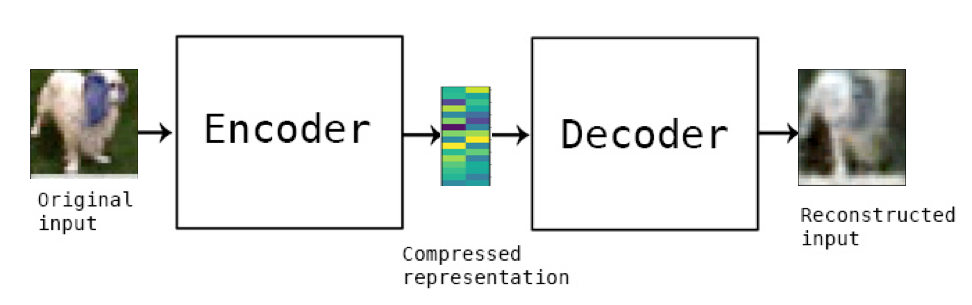
\includegraphics[width=.40\linewidth]{images/transferLearningAE}%
% }\hspace{0.5cm}
% \subfloat[one-class neural networks. \label{sfig:oc-nn-model-architecture}]{%
%   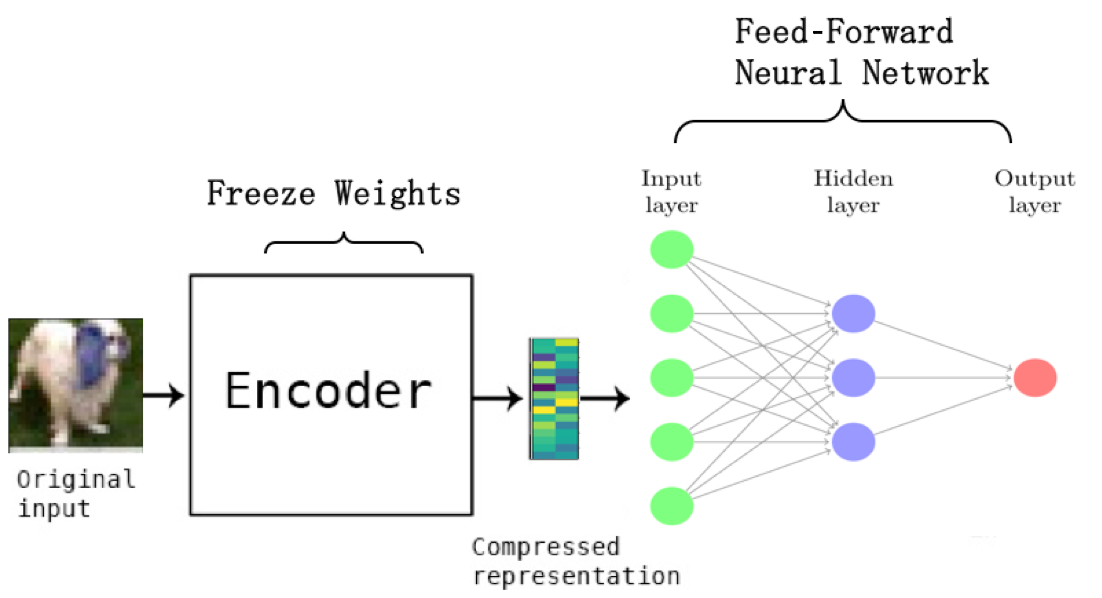
\includegraphics[width=.40\linewidth]{images/oneClassNN_model}%
% }
% \caption{Model architecture of Autoencoder  and the proposed one-class neural networks (OC-NN).}
% \label{fig:model-architecture}
% \end{figure*}
% %  End of the Figure

\begin{figure}[!t]
     \begin{subfigure}[b]{1\textwidth}
   \centering
   {\includegraphics[scale=0.50]%{catswithrotatedcats}}
{images/transferLearningAE}}
\caption{Autoencoder.}
        \end{subfigure}%
        \hfill
        \vspace{2mm}
     \begin{subfigure}[b]{1\textwidth}
\centering
   {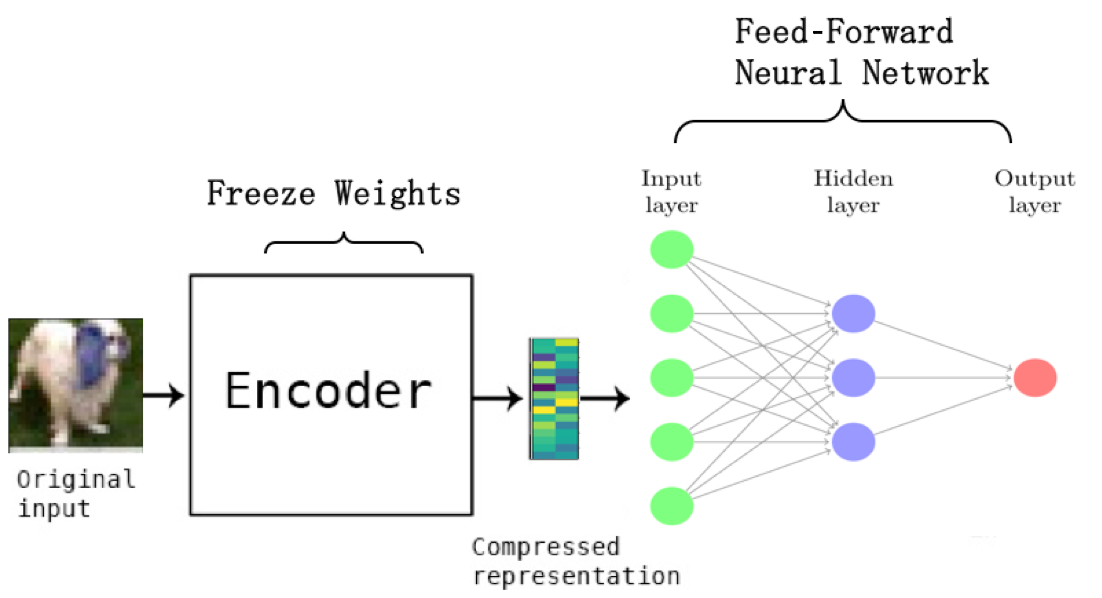
\includegraphics[scale=0.50]{images/oneClassNN_model}}
 \caption{One-class neural networks.}
        \end{subfigure}%
    \caption{
     Model architecture of Autoencoder  and the proposed one-class neural networks (OC-NN).
    }
    \label{fig:model-architecture}
\end{figure}




%Table containing the feed forward network architectures used in experiments
\begin{table}[!t]
    \centering
    \renewcommand{\arraystretch}{1.25}
    \setlength{\tabcolsep}{6pt}
    %\scalebox{0.85}{
    \begin{tabular}{@{}llll@{}}
        \toprule
        \toprule
         Dataset& \#    Input (features) & \# hidden layer( or output) \# optional layer  \\
        \toprule
        {\tt Synthetic }      & 512     & 128   & 1 \\
        {\tt MNIST}           & 32      & 32    & None \\
        {\tt CIFAR$-$10}      & 128     & 32    & None \\
        {\tt GTSRB }          & 128     & 32    & 16 \\
        \bottomrule
    \end{tabular}
    %}
    %\vspace{0.1 cm}
    \caption{Summary of best performing feed-forward network architecture's used in OC-NN model for experiments.}
    \label{tbl:feed-forward-OC-NN}
    \vspace{-\baselineskip}
\end{table}
% end of the table



































\section{Experimental results}
\label{sec:experiment-results}
\section{Experimental Results}
\label{sec:experiment-results}
In this section, we explore a variety of GAD experiments. As anomaly detection is an unsupervised learning problem, model evaluation is highly challenging. {  We employ anomaly injection where known group anomalies are injected into  real-world image datasets. The performances of DGMs are evaluated against state-of-the-art GAD methods using area under precision-recall curve (AUPRC) and area under receiver operating characteristic curve (AUROC) metrics. AUPRC  is  more appropriate  than AUROC for binary classification under class imbalanced datasets such as in GAD applications~\cite{Davis:2006}.
However in the following experiments, a high AUPRC score usually indicates the effectiveness of accurately identifying regular groups while AUROC accounts for the false positive rate of detection methods. %detection of group anomalies
}

\subsection{Synthetic Data: Rotated Gaussians }
Firstly we generate synthetic data where
regular behaviour consists of  bivariate Gaussian samples while anomalous groups have rotated covariance structures. %$\big({X}_{i1}(t),{X}_{i2}(t) \big)_{i=1}^N \sim \mathcal{N}\big ({\boldsymbol \mu(t)},\boldsymbol \Sigma(t) \big)$. In this experiment,
We generate synthetic data with number of groups $M=550$ and $M=5050$. 50 anomalous groups are injected with correlation $\rho =-0.7$ while the rest of the regular group distributions have  correlation $\rho =0.7$.  The mean vectors are randomly sampled from uniform distributions %with $  \mu_1(t), \, \mu_2(t) \sim \mathcal{U}(0,1)$ for $t \in [1,T]$.
 while covariances of group distributions are given by
 \begin{equation}
  \boldsymbol\Sigma_m=\left\{
  \begin{array}{@{}ll@{}}
  \;
\begin{pmatrix}
     0.2 & 0.14 \\
  0.14 & 0.2
  \end{pmatrix}, & m=1,2,\dots,500 \\[5mm]
  \;  \small \begin{pmatrix}
     0.2 & -0.14 \\
  -0.14 & 0.2
  \end{pmatrix}, &m=501,502,\dots,550 \end{array}\right.
    \label{changecovariance}
\end{equation}
with each group having $N_m = 1536$ observations.
{  Since we configured the proposed DGMs with an architecture suitable  for $32\times 32$ pixels for 3 dimensions (red, green, blue), our dataset is constructed such that each group has bivariate observations with a total of $N_m \times 2 = 3072$ values. }

% Equivalently, this GSP over $[1,T/2]$ has a linear correlation between observations of $\rho =0.5$ whereas there is an increase in   correlation  with $\rho =0.95$ for $(T/2,T]$. \\
% detecting tigers within cats


\textbf{Parameter settings}:
GAD methods are applied on the raw data with various parameter settings.
MGM is trained with $T=1$ regular scene types and $L=3$ as the number of Gaussian mixtures. The expected proportion of group anomalies as true proportion in OCSMM and OCSVM is set to  $\nu = 50/M$ where $M= 550$ or $M= 5050$. In addition, OCSVM is applied by treating each group as a single high-dimensional vector.

\textbf{Results}: Table \ref{tbl:syn} illustrates the results of detecting distribution-based group anomalies for different { number of groups}. For smaller {  number of groups} $M= 550$, state-of-the-art GAD methods achieve a higher performance  than DGMs however for a larger training set with $M= 5050$, deep generative models achieve the highest performance. This conveys that DGMs require larger {  number of group} observations in order to train an appropriate model. { AAE and VAE attain similar results for both synthetic datasets.}

\begin{table*}
    \centering
    \scalebox{1}{
    \begin{tabular}{|c|c|c|c|c|c|c|}
        \hline
        \multirow{2}{*}{Methods} &
        \multicolumn{2}{c|}{\bf { M=550}} &
            \multicolumn{2}{c|}{\bf { M=5050}}
        \\
        \cline{2-5}
        &AUPRC & AUROC &AUPRC & AUROC
          \\
        \hline
        AAE &$0.9060$ &$0.5000$ &\cellcolor{gray!25}$1.0000$ &\cellcolor{gray!25}$1.0000$ \\
        VAE &$0.9001$ &$0.5003$ &\cellcolor{gray!25}$1.0000$&\cellcolor{gray!25}$1.0000$ \\
%         CAE &$0.9070$ &$0.5019$ &$0.9989$&$0.9979$\\
        \midrule
        MGM&\cellcolor{gray!25}$0.9781$ &\cellcolor{gray!25}$0.8180$
           &$0.9978$ &$0.8221$\\
        OCSMM&$0.9426$ &$0.6097$%  &$0.0000$
                  &$0.9943$ &$0.6295$
        \\
        OCSVM&$0.9211$ &$0.5008$&$0.9898$ &$0.5310$%  &$0.0000$
        \\
        \hline
\end{tabular}}
       \vspace{2mm}
        \caption{Results for detecting rotated Gaussian distributions in synthetic datasets where % the first two rows contains deep generative models (AAE and VAE) while other techniques are state-of-the-art GAD methods.
        AAE and VAE attain poor detection results for smaller datasets while they achieve highest performances (as highlighted in gray) for a larger number of groups.  }
    \label{tbl:syn}
\end{table*}

\subsection{Detecting tigers within cat images }
\label{sec:tigerDetect}
%In this section we provide empirical results produced by DNN on synthetic and real data. We show that DNN outperforms several sate-of-the-art competitors in the group anomaly detection task.
Firstly we explore the detection of point-based group anomalies (or image anomalies) by injecting 50 anomalous images of tigers among 5000 cat images.
From Figure~\ref{fig:GAD} (a), the visual features of cats are considered as regular behaviour while  characteristics of tigers are anomalous. The goal is to correctly detect images of tigers (point-based group anomalies) in an unsupervised manner.

\textbf{Parameter settings}:
In this experiment, HOG extracts visual features as inputs for GAD methods. MGM is trained with $T=1$ regular cat type and $L=3$ as the number of mixtures. Parameters in OCSMM and OCSVM are set to  $\nu$ = 50/5050 and OCSVM is applied with $k$-means ($k=40$). Following the success of the Batch Normalisation architecture~\cite{ioffe2015batch} and Exponential Linear Units (elu)~\cite{clevert2015fast}, we have found that convolutional+batch-normalisation+elu layers for DGMs provide a better representation of convolutional filters. Hence, in this experiment the autoencoder of both AAE and VAE adopts four layers of (conv-batch-normalisation-elu) in the encoder part and as well as in the decoder portion of the network. AAE network parameters such as (number of filter, filter size, strides) are chosen to be (16,3,1) for first and second layers while (32,3,1) for third and fourth layers of both encoder and decoder layers. The middle hidden layer size is set to be same as rank $K = 64$ and the model is trained using Adam~\cite{kingma2014adam}. The decoding layer uses sigmoid function in order to capture the non-linearity characteristics from  latent representations produced by the hidden layer.  Similar parameter settings are selected for DGMs in subsequent experiments.


{
\textbf{Results}:
From Table  \ref{tablesummary}, AAE attains the highest AUROC value of 0.9906 while OCSMM achieves a AUPRC of 0.9941. MGM, OCSMM, OCSVM are associated with high AUPRC as  regular groups are correctly identified but their low AUROC scores indicate poor detection of group anomalies. Figure  \ref{fig:results-cifar} (a) further investigates the top 10 anomalous images detected by these methods and finds that AAE correctly detects all images of tigers while OCSMM erroneously captures regular cat images.
}


% detecting cats with dogs
\subsection{Detecting cats and dogs }
We further investigate GAD  %of distribution-based group anomalies
where images of a single cat and dog are considered as regular groups while  images with both cats and dogs are distribution-based group anomalies.   The constructed dataset consists of 5050 images; 2500 single cats, 2500 single dogs and 50 images of  cats and dogs together. % Examples of anomalous images containing  cats and dogs together are previously illustrated in Figure~\ref{fig:GAD}(B).
As previously illustrated in Figure~\ref{fig:GAD} (b), our goal is to detect all images with irregular mixtures of cats and dogs in an unsupervised manner.

% Results for Detecting Cats and Rotated Cats along with detecting Cats together with Dogs.
\textbf{Parameter settings}:
In this experiment, HOG extracts visual features as inputs for GAD methods.
MGM is trained with $T=2$ regular cat type and $L=3$ as the number of mixtures while  OCSVM is applied with $k$-means ($k=30$).

{
\textbf{Results}:
Table  \ref{tablesummary} highlights (in gray) that AEE achieves the highest  AUPRC and AUROC values. %AAE and VAE achieve similar detection performances with AUROC of 1 and 0.9999 respectively. %%%  Why are they similar? Can we know?
Other state-of-the-art GAD methods attain high AUPRC however AUROC values are relatively low. From Figure  \ref{fig:results-cifar} (a), the top 10 anomalous images with both cats and dogs are correctly detected by AAE while OCSMM erroneously captures regular cat images. In fact, OCSMM incorrectly but consistently detects regular cats with similar results to subsection~\ref{sec:tigerDetect}.

}







\subsection{Discovering rotated entities }
We now explore the detection of distribution-based group anomalies with  5000  regular cat images and 50 images of rotated cats. As illustrated in Figure~\ref{fig:GAD} (a), images of rotated cats are anomalous  compared to regular images of cats. Our goal is to detect all rotated cats in an unsupervised manner.

\textbf{Parameter settings}:
In this experiment involving rotated entities, HOG extracts visual features  because SIFT is rotation invariant. MGM is trained with $T=1$ regular cat type and $L=3$ mixtures  while OCSVM is applied with $k$-means ($k=40$).  %For the DGMs, the network parameters follows similar settings to subsection \ref{sec:tigerDetect}. % previous experiment of detecting tigers within cats images.

{
\textbf{Results}:
 In  Table  \ref{tablesummary}, AAE and VAE achieve the highest AUROC with AAE having slightly better detection results. MGM, OCSMM and OCSVM achieve a high AUPRC but low AUROC. Figure \ref{fig:results-rotatedcatsandscene} (a) illustrates the  top 10 most anomalous groups where AAE correctly detects images containing rotated cats while MGM incorrectly identifies regular cats as anomalous. }


\begin{figure}[!t]
     \begin{subfigure}[b]{1\textwidth}
   \centering
   {\includegraphics[scale=0.50]%{catswithrotatedcats}}
{Tigers}}
\caption{Tigers within cat images from {\tt cifar-10} dataset.}
        \end{subfigure}%
        \hfill
        \vspace{2mm}
     \begin{subfigure}[b]{1\textwidth}
\centering
   {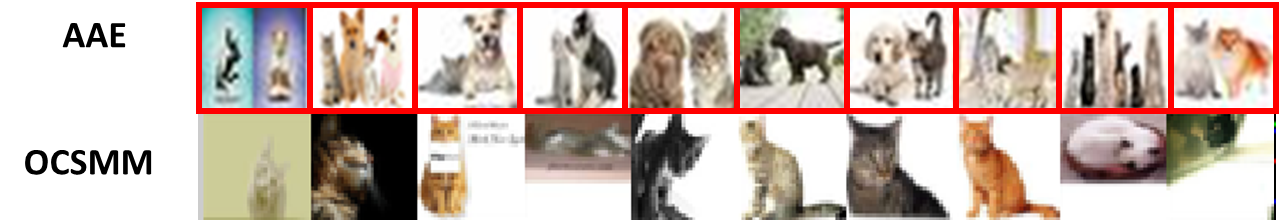
\includegraphics[scale=0.50]{CatsAndDogs}}
\caption{Images of cats and  dogs within single cat and dog images using {\tt cifar-10} dataset.}
        \end{subfigure}%
    \caption{
    Top 10 anomalous groups are presented for AAE and the best GAD method respectively where red boxes outlining images represent true group anomalies.
    %Red boxes around images  represent correctly detected group anomalies as shown in (a) and (b).
    AAE  has an accurate detection of anomalous tigers injected into the {\tt cifar-10} dataset as well as for anomalous images of both cats and dogs. On the other hand, OCSMM consistently but erroneously identifies similar cat images as the most anomalous groups.
    }
    \label{fig:results-cifar}
\end{figure}




% Detecting Stitched scene images.
\subsection{Detecting stitched scene images}
A scene image dataset is also explored where %the two datasets described in Section \ref{sec:experiment-setup}.
 100 images from each category ``inside city”, ``mountain" and ``coast”. 66 group anomalies are added where images are stitched from  two scene categories. % These 300 images are randomly divided: 80\% are used for training and the rest for testing.
% We created anomalies by stitching random regular images from two  categories.
Illustrations are provided in Figure~\ref{fig:GAD} (c) where a stitched image may contain half coast and half city street view. These anomalies are challenging to detect since they have the same local features as regular images however as a collection, they are anomalous.  Our objective is detect stitched scene images in an unsupervised manner.

\textbf{Parameter settings}:
State-of-the-art GAD methods utilise SIFT feature extraction in this experiment. MGM is trained with $T=3$ regular scene types and $L=4$ Gaussian mixtures while %. The expected proportion of group anomalies as true proportion in OCSMM and OCSVMM is set to  $\nu$ = 66/366 where
OCSVM is applied with $k$-means ($k=10$). The scene image dimensions are rescaled
to enable the application of an identical architecture for DGMs as implemented in previous experiments. %
The parameter settings for both AAE and VAE  follows setup as described in Section~\ref{sec:tigerDetect}.

{
\textbf{Results}:
In Table  \ref{tablesummary}, OCSMM achieves the highest AUROC score  %attains the highest performance with AUROC of 0.7162  while AAE has a AUPRC of 0.9449.
%Many GAD methods outperform DGMs in this experiment as
while DGMs are less effective in detecting distribution-based group anomalies in this experiment. We suppose that this is because  only $M=366$ groups are available for training in the  {\tt scene} dataset as  compared to $M=5050$ groups in previous experiments.  Figure  \ref{fig:results-rotatedcatsandscene}   (b) displays the top 10 most anomalous images where OCSMM achieves a better detection results % of distribution-based group anomalies
than AAE.
}

\begin{figure}[!t]
    \centering
 \begin{subfigure}[b]{1\textwidth}
\centering
   {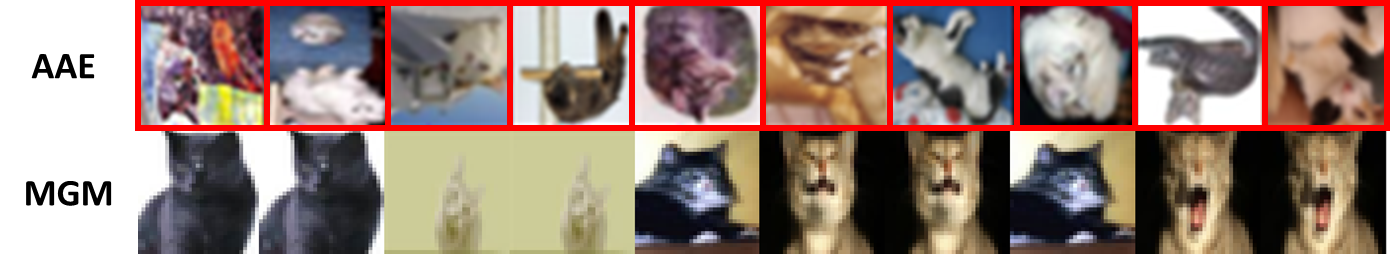
\includegraphics[scale=0.47]{RotatedCats}}
\caption{Rotated cats  amongst regular cats in the {\tt cifar-10} dataset. }
 \end{subfigure}%
 \hfill \vspace{2mm}
 \begin{subfigure}[b]{1\textwidth}
\centering
 {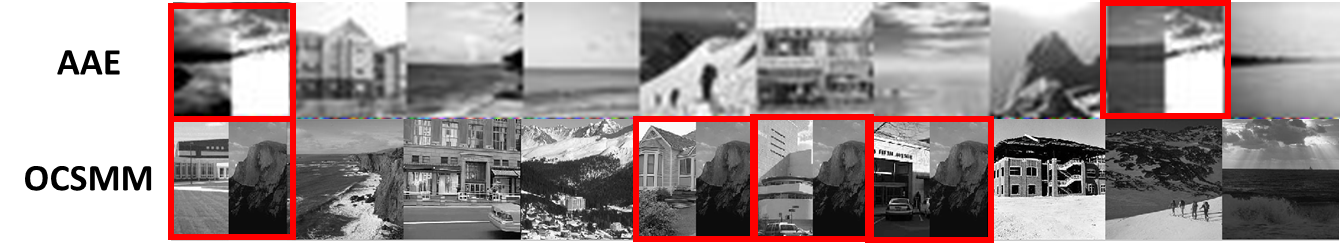
\includegraphics[scale=0.5]{Scene}}
\caption{Stitched Images amongst the {\tt scene} dataset.}
        \end{subfigure}%
   \caption{Top 10 anomalous groups are presented where red boxes outlining images  represent true group anomalies in the given datasets. AAE performs well in (a) with number of groups $M=5050$ however does not effectively detect group anomalies in (b) where number of groups is $M=366$.  MGM is unable to correctly detect any rotated cats while OSCMM is able to group anomalies in the {\tt scene} dataset.
   }
    \label{fig:results-rotatedcatsandscene}
\end{figure}



\subsection{ Results Summary and Discussion}

Table  ~\ref{tablesummary} summarises the performance of detection methods in
%DGMs and state-of-the-art GAD methods for
 our experiments.
AAE usually achieves better results than VAE as AAE has the  advantage of the embedding coverage in the latent space~\cite{makhzani2015adversarial}.  AAE enforces a better mapping of input variables to embedding space and hence captures more robust input features.
DGMs have a significantly worse performance on  {\tt synthetic} and {\tt scene} datasets due to the small number of groups. A high detection performance is achieved for larger number of groups with {\tt cifar-10} and {\tt Pixabay} data experiments.
 Overall, given a sufficient number of group observations for training, DGMs are effective in detecting group anomalies however poor detection occurs for datasets with a small number of groups.







\begin{table*}
   % \centering
        \setlength{\tabcolsep}{1.2mm}
    \scalebox{1}{
    \begin{tabular}{|c|c|c|c|c|c|c|c|c|c|c|}

        \hline
        \multirow{2}{*}{Methods} &
        \multicolumn{2}{c|}{\bf {\small    Tigers }}  &
                \multicolumn{2}{c|}{\bf {\small Cats and Dogs }} &
                \multicolumn{2}{c|}{\bf {\small Rotated Cats}} &
                                  \multicolumn{2}{c|}{\bf {\small Scene }} \\[1mm]
        \cline{2-9}
     &AUPRC & AUROC        & AUPRC & AUROC      &AUPRC & AUROC        & AUPRC & AUROC
        \\
        \hline
        \multirow{4}{*}{}
        AAE& $0.9449$ &\cellcolor{gray!25} $0.9906$
         &\cellcolor{gray!25}$1.0000$ &\cellcolor{gray!25}$1.0000$
            &\cellcolor{gray!25}$1.0000$ &\cellcolor{gray!25}$1.0000$
        & \cellcolor{gray!25} 0.9449 & 0.5906
        \\
          %      AAE\cite{chalapathy2017robust}&\cellcolor{gray!25}$1.0000$ &\cellcolor{gray!25}$1.0000$
                %&\cellcolor{gray!25}$1.0000$                   &\cellcolor{gray!25}$1.0000$ &\cellcolor{gray!25}$1.0000$%&\cellcolor{gray!25}$1.0000$           \\
%         CAE & &
%         &$0.9998$ &$0.9999$
%          &$0.9999$ &$0.9999$
%         & &
%         \\
        VAE&$0.9786$ &$0.9092$ % &$0.9997$
               &$0.9998$ &$0.9999$
        &$0.9999$ &$0.9999$%&$0.9999$
                  &$0.8786$ &$0.3092$
        \\
        \midrule
        MGM & $0.9881$ & $0.5740$
        &0.9906 & 0.5377
        &$0.9919$ &$0.6240$ % &$0.0000$
               &0.8835 & 0.6639
        \\
        OCSMM
             &\cellcolor{gray!25} $0.9941$ &$0.6461$%  &$0.0000$
        & 0.9930 & 0.5876
        &$0.9917$ &$0.6128$%  &$0.0000$
             &$0.9140$ &\cellcolor{gray!25} $0.7162$%  &$0.0000$
        \\
        OCSVM
        & 0.9909 & 0.5474
        & 0.9916 & 0.5549
        &$0.9894$ &$0.5568$%  &$0.0000$
        & 0.8650 & 0.5733
        \\
        \hline
\end{tabular}}
       \vspace{2mm}
        \caption{Summary of results for various data experiments where first two rows contains deep generative models and other techniques are state-of-the-art GAD methods. The highest values of performance metrics are shaded in gray.}
    \label{tablesummary}
\end{table*}


{\bf Comparison of training times:}
\label{sec:runtime}
We add a final remark about applying the proposed DGMs on  GAD problems in terms of computational time and training efficiency.
For example, including the time taken to calculate SIFT features on the small-scale {\tt scene} dataset, MGM takes 42.8 seconds for training, 3.74 minutes to train OCSMM and 27.9 seconds for OCSVM. In comparison, the computational times for our AAE and VAE are  6.5 minutes and 8.5 minutes respectively. %All the experiments involving DGMs were conducted on a MacBook Pro equipped with an Intel Core i7 at 2.2 GHz, 16 GB of RAM (DDR3 1600 MHz).
 The ability to leverage recent advances in deep learning as part of our optimisation (e.g. training models on a GPU) is  a salient feature of our approach. We also note that MGM and OCSMM are faster to train on small-scale datasets however they suffer from at least $O(N^2)$ complexity for total number of observations $N$. %; for example, it takes over an hour to train on the {\tt cifar-10} dataset.
It is plausible that one could leverage recent advances in fast approximations of kernel methods~\cite{Lopez-Paz:2014} for OCSMM and studying these would be of interest in future work.











\section{Conclusion}
\label{sec:conclusion}
% !TEX root=../main.tex
\section{Conclusion}
\label{sec:ocnn_conclusion}
In this paper, we have proposed a one-class neural network (OC-NN) approach for anomaly detection.
OC-NN uses a one-class SVM (OC-SVM) like loss function to train a neural network.
The advantage of OC-NN is that the features of the hidden layers are constructed for the specific
task of anomaly detection. This approach is substantially different from recently proposed
hybrid approaches which use deep learning features as input into an anomaly detector.  Feature
extraction in hybrid approaches is generic and not aware of the anomaly detection task. To learn
the parameters of the OC-NN network we have proposed a novel alternating minimization approach and
have shown that the optimization of a subproblem in OC-NN is equivalent to a quantile selection
% problem. Experiments on complex image and sequential data sets demonstrates that OC-NN is
% highly accurate. For future work, we would like to build and deploy an end to end system for anomaly
% detection based on OC-NN.




\bibliographystyle{splncs03}
\bibliography{MyBibFile,outlier}

\end{document}
